\documentclass[a4paper, oneside]{book}

\usepackage{graphicx} % allows inserting graphics
\usepackage{listings}
\usepackage{algpseudocode} % allows code snippets
\usepackage{algorithm}
\usepackage{hyperref} % allows
\usepackage{subcaption} 
\usepackage[export]{adjustbox} 
\usepackage{wrapfig} % allows warped figures
\usepackage[acronym]{glossaries} % add glossary
\usepackage{acronym} % add acronyms
\usepackage{subfiles} % support multiple files
\usepackage{fancyhdr} % more control on headers and footers
\usepackage{xcolor}
\usepackage[italian]{babel}

\usepackage{arydshln}
\usepackage{multirow}
\usepackage{titlesec}

\usepackage{tcolorbox}
\usepackage{multicol}
\usepackage{xcolor}
\usepackage{tikz}

% Define a helper for the hswatch
\newcommand{\hswatch}[1]{%
    \definecolor{tmp}{HTML}{#1}%
    \smash{\tikz[baseline=-0.6ex]\node[fill=tmp, draw=black, line width=0.1mm, minimum size=3.5mm, rounded corners=1pt]{};}%
}


\titleformat{\chapter}[hang] 
{\normalfont\huge\bfseries}{\thechapter}{1em}{}

\graphicspath{ {./images/} }

\pagestyle{plain}

\begin{document}

\begin{titlepage}
    
    \noindent
    \begin{minipage}[t]{0.19\textwidth}
        \vspace{-4mm}{
\includegraphics[scale=1.10]{images/logo_unimib.pdf}}
    \end{minipage}
    \hspace{2mm}
    \begin{minipage}[t]{0.70\textwidth}
    {
            {\textsc{Università degli Studi di Milano - Bicocca}} \\
            \textbf{Dipartimento di Informatica, Sistemistica e Comunicazione} \\
            \textbf{Corso di Laurea in Informatica} \\
            \par
    }
    \end{minipage}
    
\vspace{40mm}
    
\begin{center}
        {\LARGE{
                \textbf{ Presentazione Stage  }
                \par
        }}
    \end{center}
    
    \vspace{50mm}

    
    \vspace{15mm}

    \begin{flushright}
        \large{ Maksym Naumenko } \\
        \large{ Matricola 899645 } 
    \end{flushright}
    
    \vspace{20mm}
    \begin{center}
        {\large{\bf Anno Accademico 2025-2026}}
    \end{center}

\end{titlepage}


\tableofcontents

\chapter{Cardinalità delle classi}

\begin{table}[h!]
    \centering
    \caption{quante volte ciascuna delle 26 classe appare in un'immagine distinta vs quante istanze ci sono in totale di ciascuna classe}
    \label{tab:data}
    \begin{tabular}{|l|l|l|}
        \hline
         & immagini & istanze \\ \hline
        food & 55 & 413 \\ \hline
        snack & 37 & 65 \\ \hline
        sweets & 17 & 17 \\ \hline
        fork & 56 & 82 \\ \hline
        spoon & 36 & 69 \\ \hline
        knife & 29 & 36 \\ \hline
        disposable cutlery & 12 & 12 \\ \hline
        napkin & 98 & 200 \\ \hline
        plastic bottle & 37 & 78 \\ \hline
        crushed plastic bottle & 8 & 8 \\ \hline
        alluminum can & 34 & 69 \\ \hline
        thermal bottle & 22 & 67 \\ \hline
        tetrapak & 26 & 54 \\ \hline
        glass bottle & 24 & 24 \\ \hline
        yogurt & 27 & 27 \\ \hline
        plastic cup & 41 & 77 \\ \hline
        mug & 22 & 22 \\ \hline
        oil cruet & 26 & 26 \\ \hline
        tissues & 30 & 40 \\ \hline
        keys & 27 & 27 \\ \hline
        wallet & 14 & 14 \\ \hline
        salt shaker & 17 & 17 \\ \hline
        phone & 18 & 18 \\ \hline
        earbuds & 21 & 34 \\ \hline
        lighter & 24 & 38 \\ \hline
        lip balm & 20 & 43 \\ \hline
        cigarettes & 10 & 10 \\ \hline
    \end{tabular}
\end{table}

\begin{table}[h!]
    \centering
    \caption{valori medi della Tabella \ref{tab:data} tralasciando la classe 'food'}
    \label{tab:meandata}
    \begin{tabular}{|l|l|l|}
        \hline
         & immagini & istanze \\ \hline
        media di 25 classi & 28.2 & 45.2 \\ \hline
    \end{tabular}
\end{table}

\chapter{Strategie di training}

\begin{table}[h!]
    \centering
    \caption{}
    \label{tab:strategies}
    \begin{tabular}{|l|l|l|l|l|}
        \hline
        &                   & istante & training                      & test \\ \hline
        1 & vanilla         & $t_0$   & Coke $\rightarrow$ Coke       & Coke $\rightarrow$ Coke \\ \hline
        
        % {3}{*} spans 3 lines. The * auto-adjusts width. 
        \multirow{3}{*}{2}  & \multirow{3}{*}{LWF (new class)} & $t_0$ & Coke $\rightarrow$ Coke & Coke $\rightarrow$ Coke \\ \cdashline{3-5}
        &                   & $t_1$   & Fanta $\rightarrow$ Fanta     & Coke $\rightarrow$ Coke \\ 
        &                   &         &                               & Fanta $\rightarrow$ Fanta \\ \hline
        
        \multirow{3}{*}{3}  & \multirow{3}{*}{LWF (same classes)} & $t_0$ & Coke $\rightarrow$ Alluminum  & Coke $\rightarrow$ Alluminum \\ \cdashline{3-5}
        &                   & $t_1$   & Fanta $\rightarrow$ Alluminum & Coke $\rightarrow$ Alluminum \\ 
        &                   &         &                               & Fanta $\rightarrow$ Alluminum \\ \hline
        
        \multirow{2}{*}{4} & \multirow{2}{*}{baseline per approccio \#3} & $t_0$ & Coke $\rightarrow$ Alluminum & Coke $\rightarrow$ Alluminum \\
        &                   &         &                               & Fanta $\rightarrow$ Alluminum \\ \hline
    \end{tabular}
\end{table}

\chapter{Legenda Classi}

\begin{multicols}{2}
    \subsubsection*{Cibo e Snack}
    \hswatch{f800ff} Food \\
    \hswatch{4d4a79} Snack \\
    \hswatch{1a5132} Sweets \\
    \hswatch{6dab66} Yogurt 

    \subsubsection*{Posate}
    \hswatch{39342e} Fork \\
    \hswatch{625a58} Spoon \\
    \hswatch{847e87} Knife \\
    \hswatch{ffffff} Disposable Cutlery 

    \subsubsection*{Contenitori e Bottiglie}
    \hswatch{221fdb} Crushed Bottle \\
    \hswatch{273b76} Plastic Bottle \\
    \hswatch{2f4788} Aluminum Can \\
    \hswatch{365399} Thermal Bottle \\
    \hswatch{456bbb} Tetrapak \\
    \hswatch{5483dd} Glass Bottle \\
    \hswatch{5799e6} Plastic Cup \\
    \hswatch{5aafee} Mug

    \subsubsection*{Oggetti Personali}
    \hswatch{d20505} Oil Cruet \\
    \hswatch{de2d13} Tissues \\
    \hswatch{e4411a} Keys \\
    \hswatch{e95521} Wallet \\
    \hswatch{ec5f25} Salt Shaker
    \hswatch{ef6928} Phone \\
    \hswatch{f47d2f} Ear Buds \\
    \hswatch{fa9136} Lighter \\
    \hswatch{ffa43c} Lip Balm \\
    \hswatch{f8b05d} Cigarettes \\
\end{multicols}

\begin{figure}[!ht]
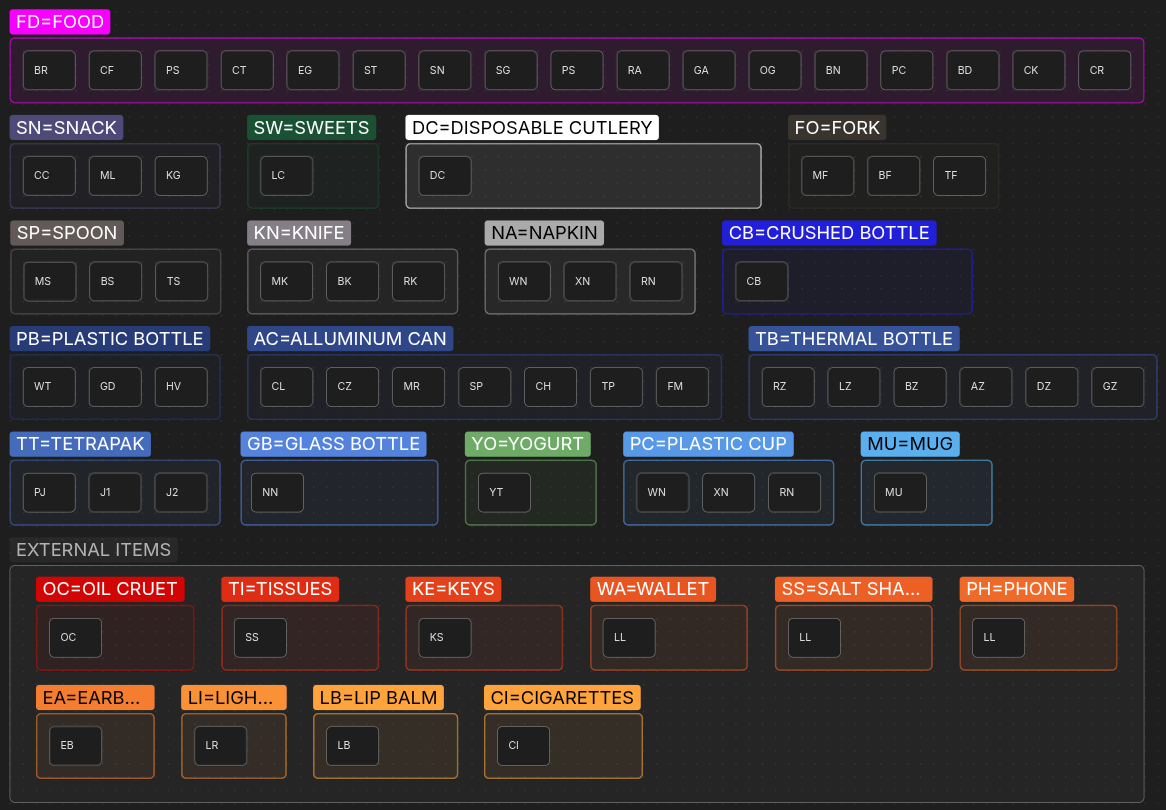
\includegraphics[width=\linewidth]{classes} 
\caption{Ogni rettangolo nero rappresenta un elemento distinto appartenente ad una classe generale (colorata)}
\label{fig:subim0}
\end{figure}

\chapter{Esempi di immagini annotate}

\begin{figure}[!ht]
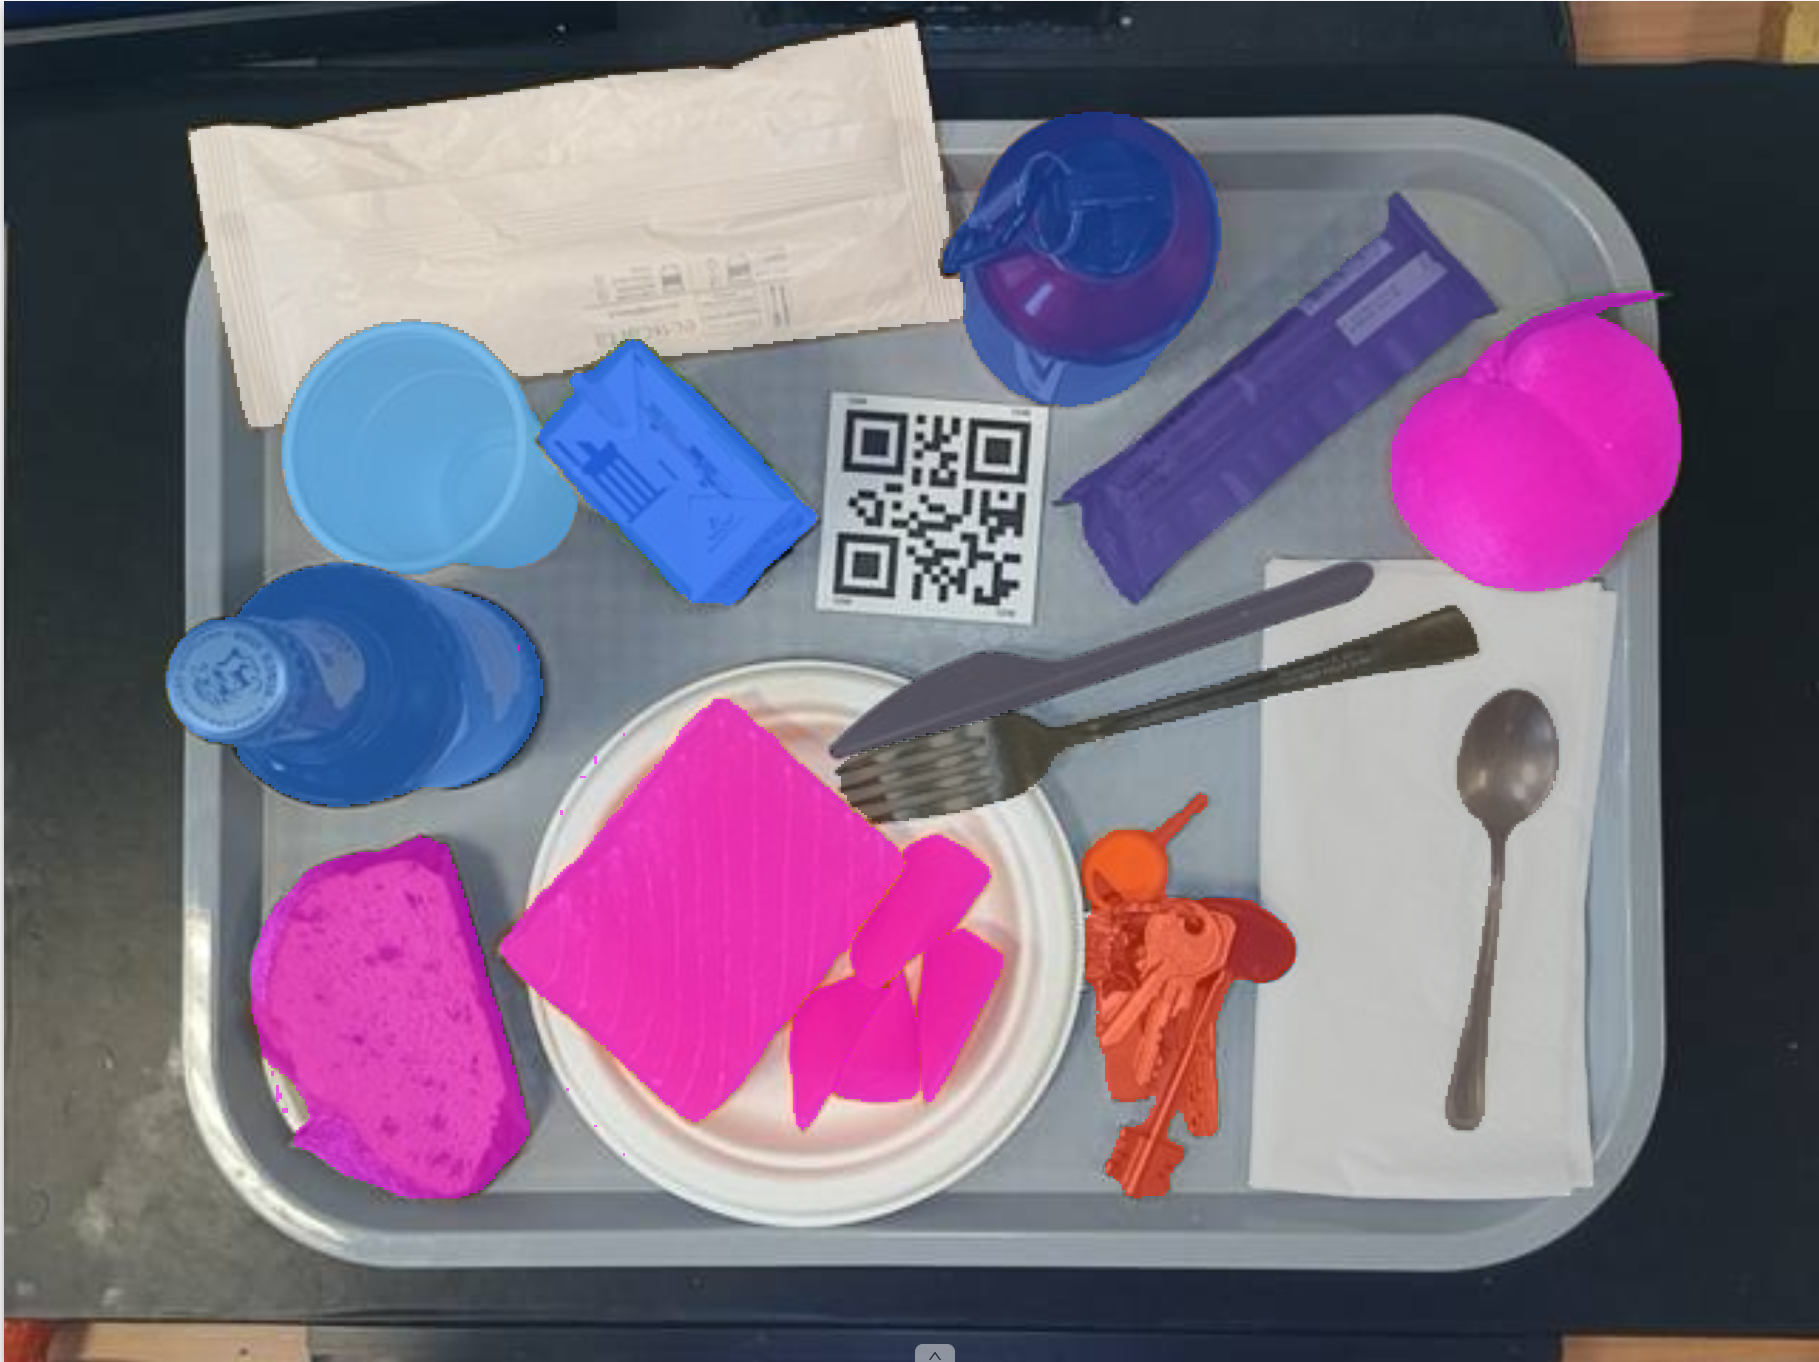
\includegraphics[width=\linewidth]{29} 
\caption{29.png}
\label{fig:subim1}
\end{figure}

\begin{figure}[!ht]
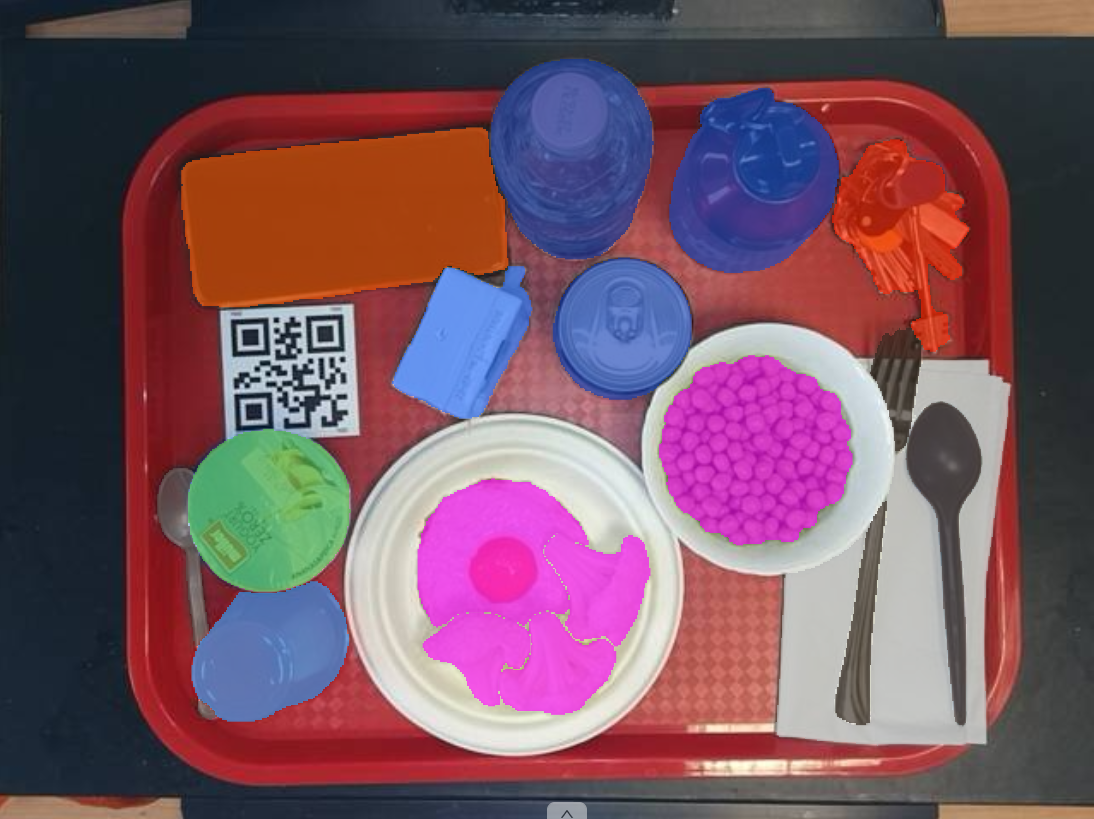
\includegraphics[width=\linewidth]{42} 
\caption{42.png}
\label{fig:subim2}
\end{figure}

\begin{figure}[!ht]
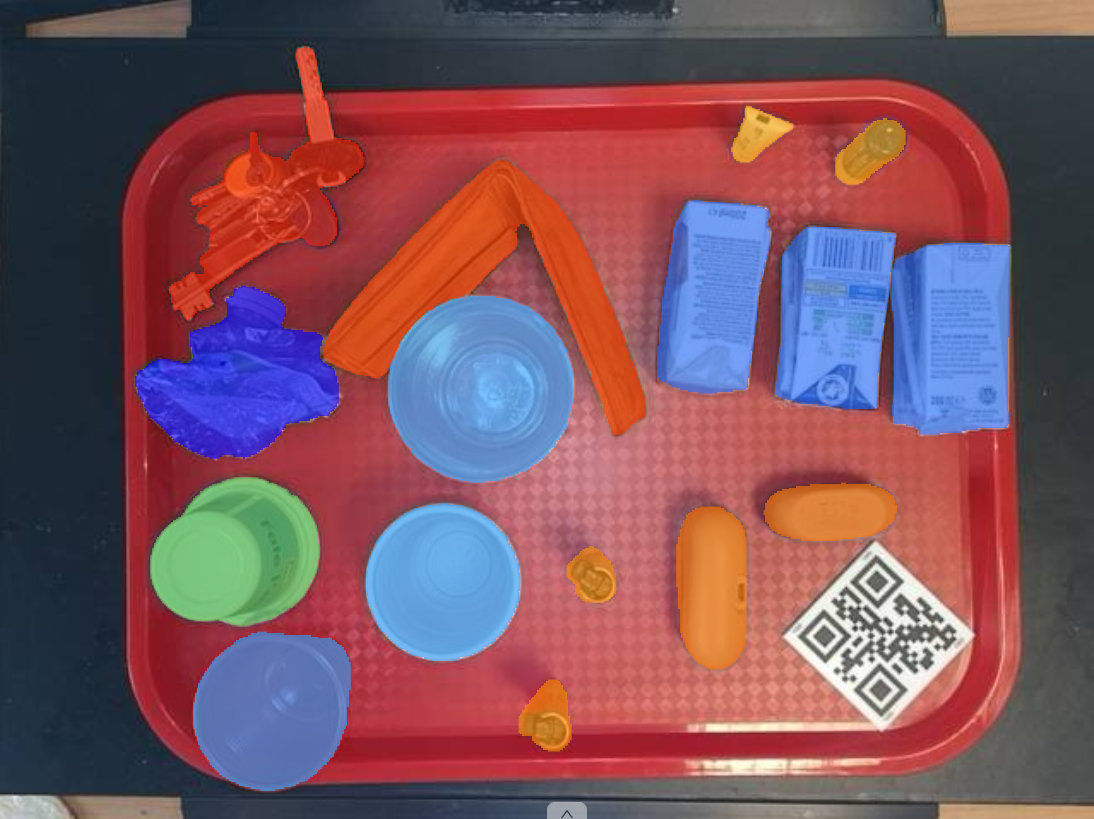
\includegraphics[width=\linewidth]{54} 
\caption{54.png}
\label{fig:subim3}
\end{figure}

\begin{figure}[!ht]
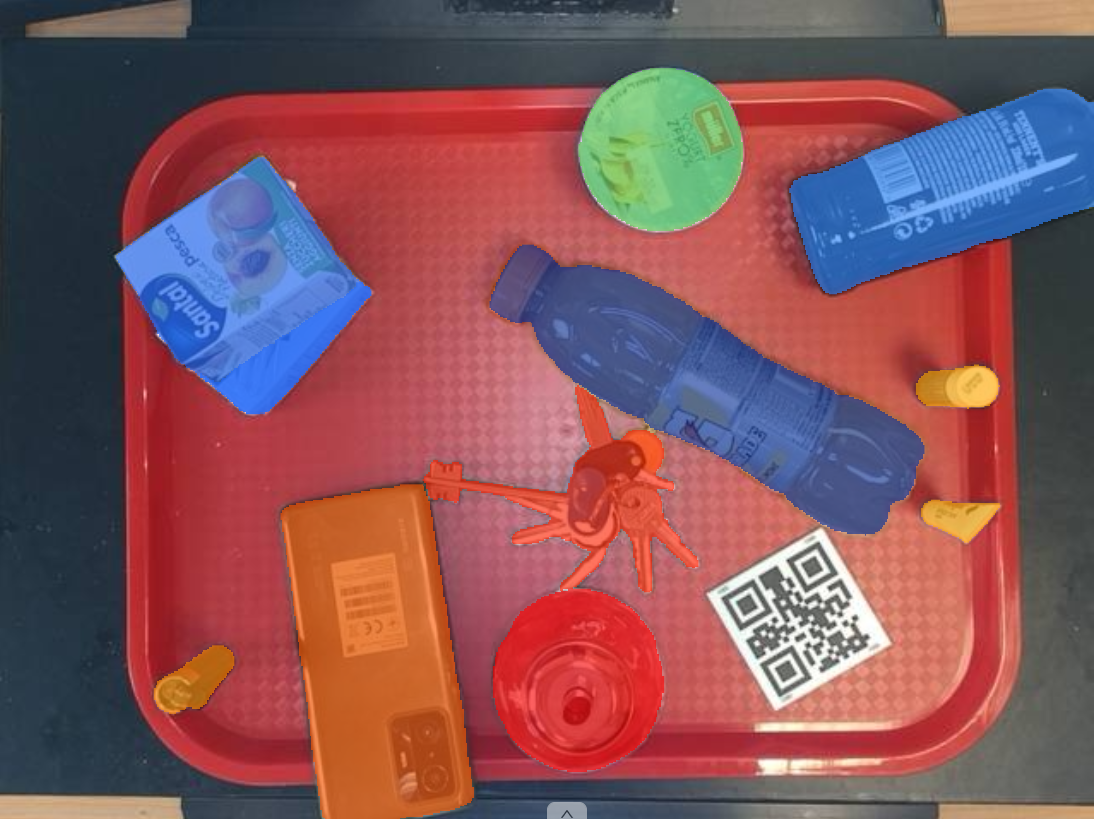
\includegraphics[width=\linewidth]{56} 
\caption{56.png}
\label{fig:subim4}
\end{figure}

\begin{figure}[!ht]
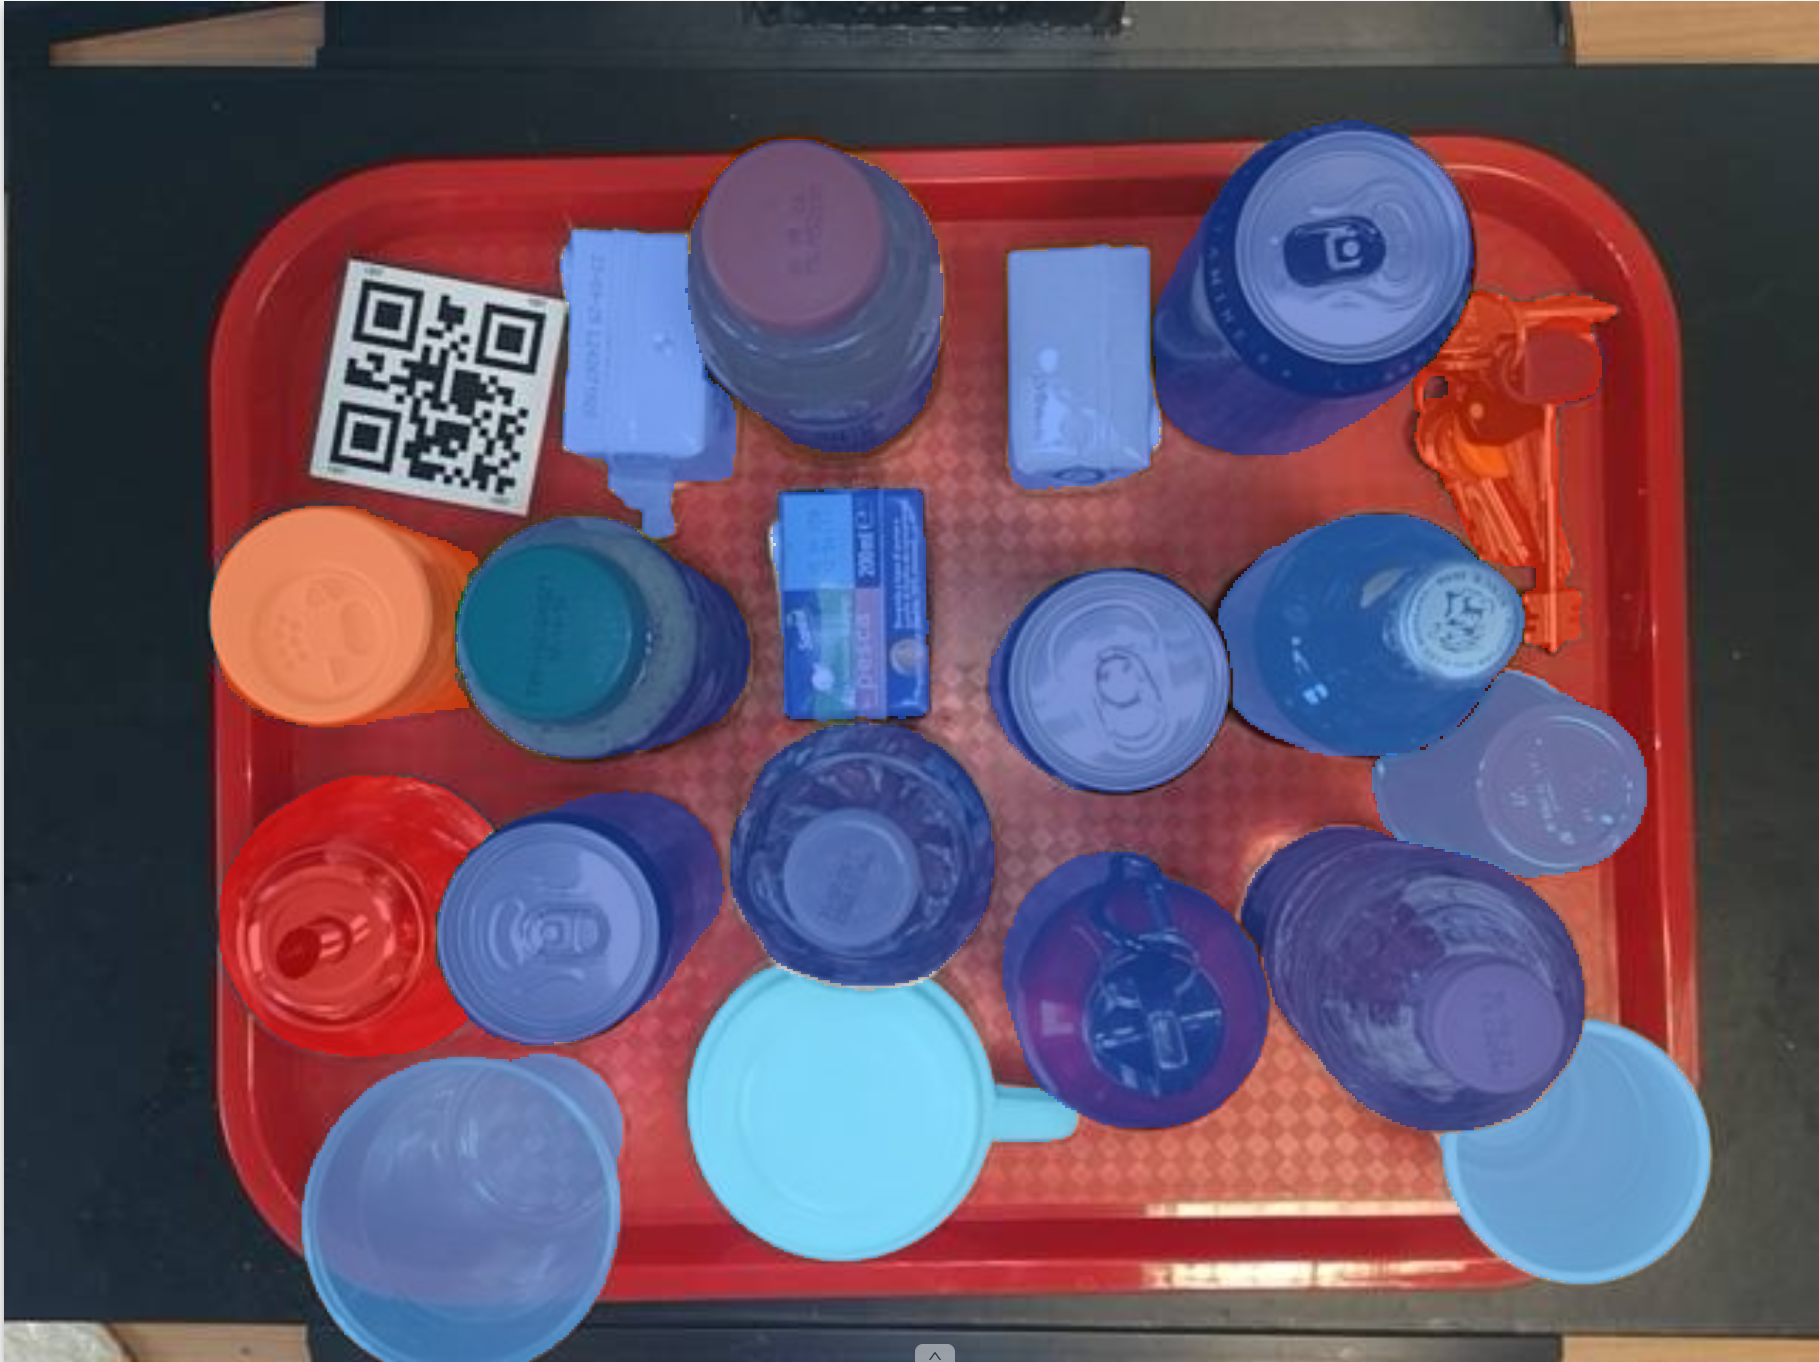
\includegraphics[width=\linewidth]{62} 
\caption{62.png}
\label{fig:subim5}
\end{figure}

\chapter{Omogeneità dataset}

\begin{figure}[!ht]
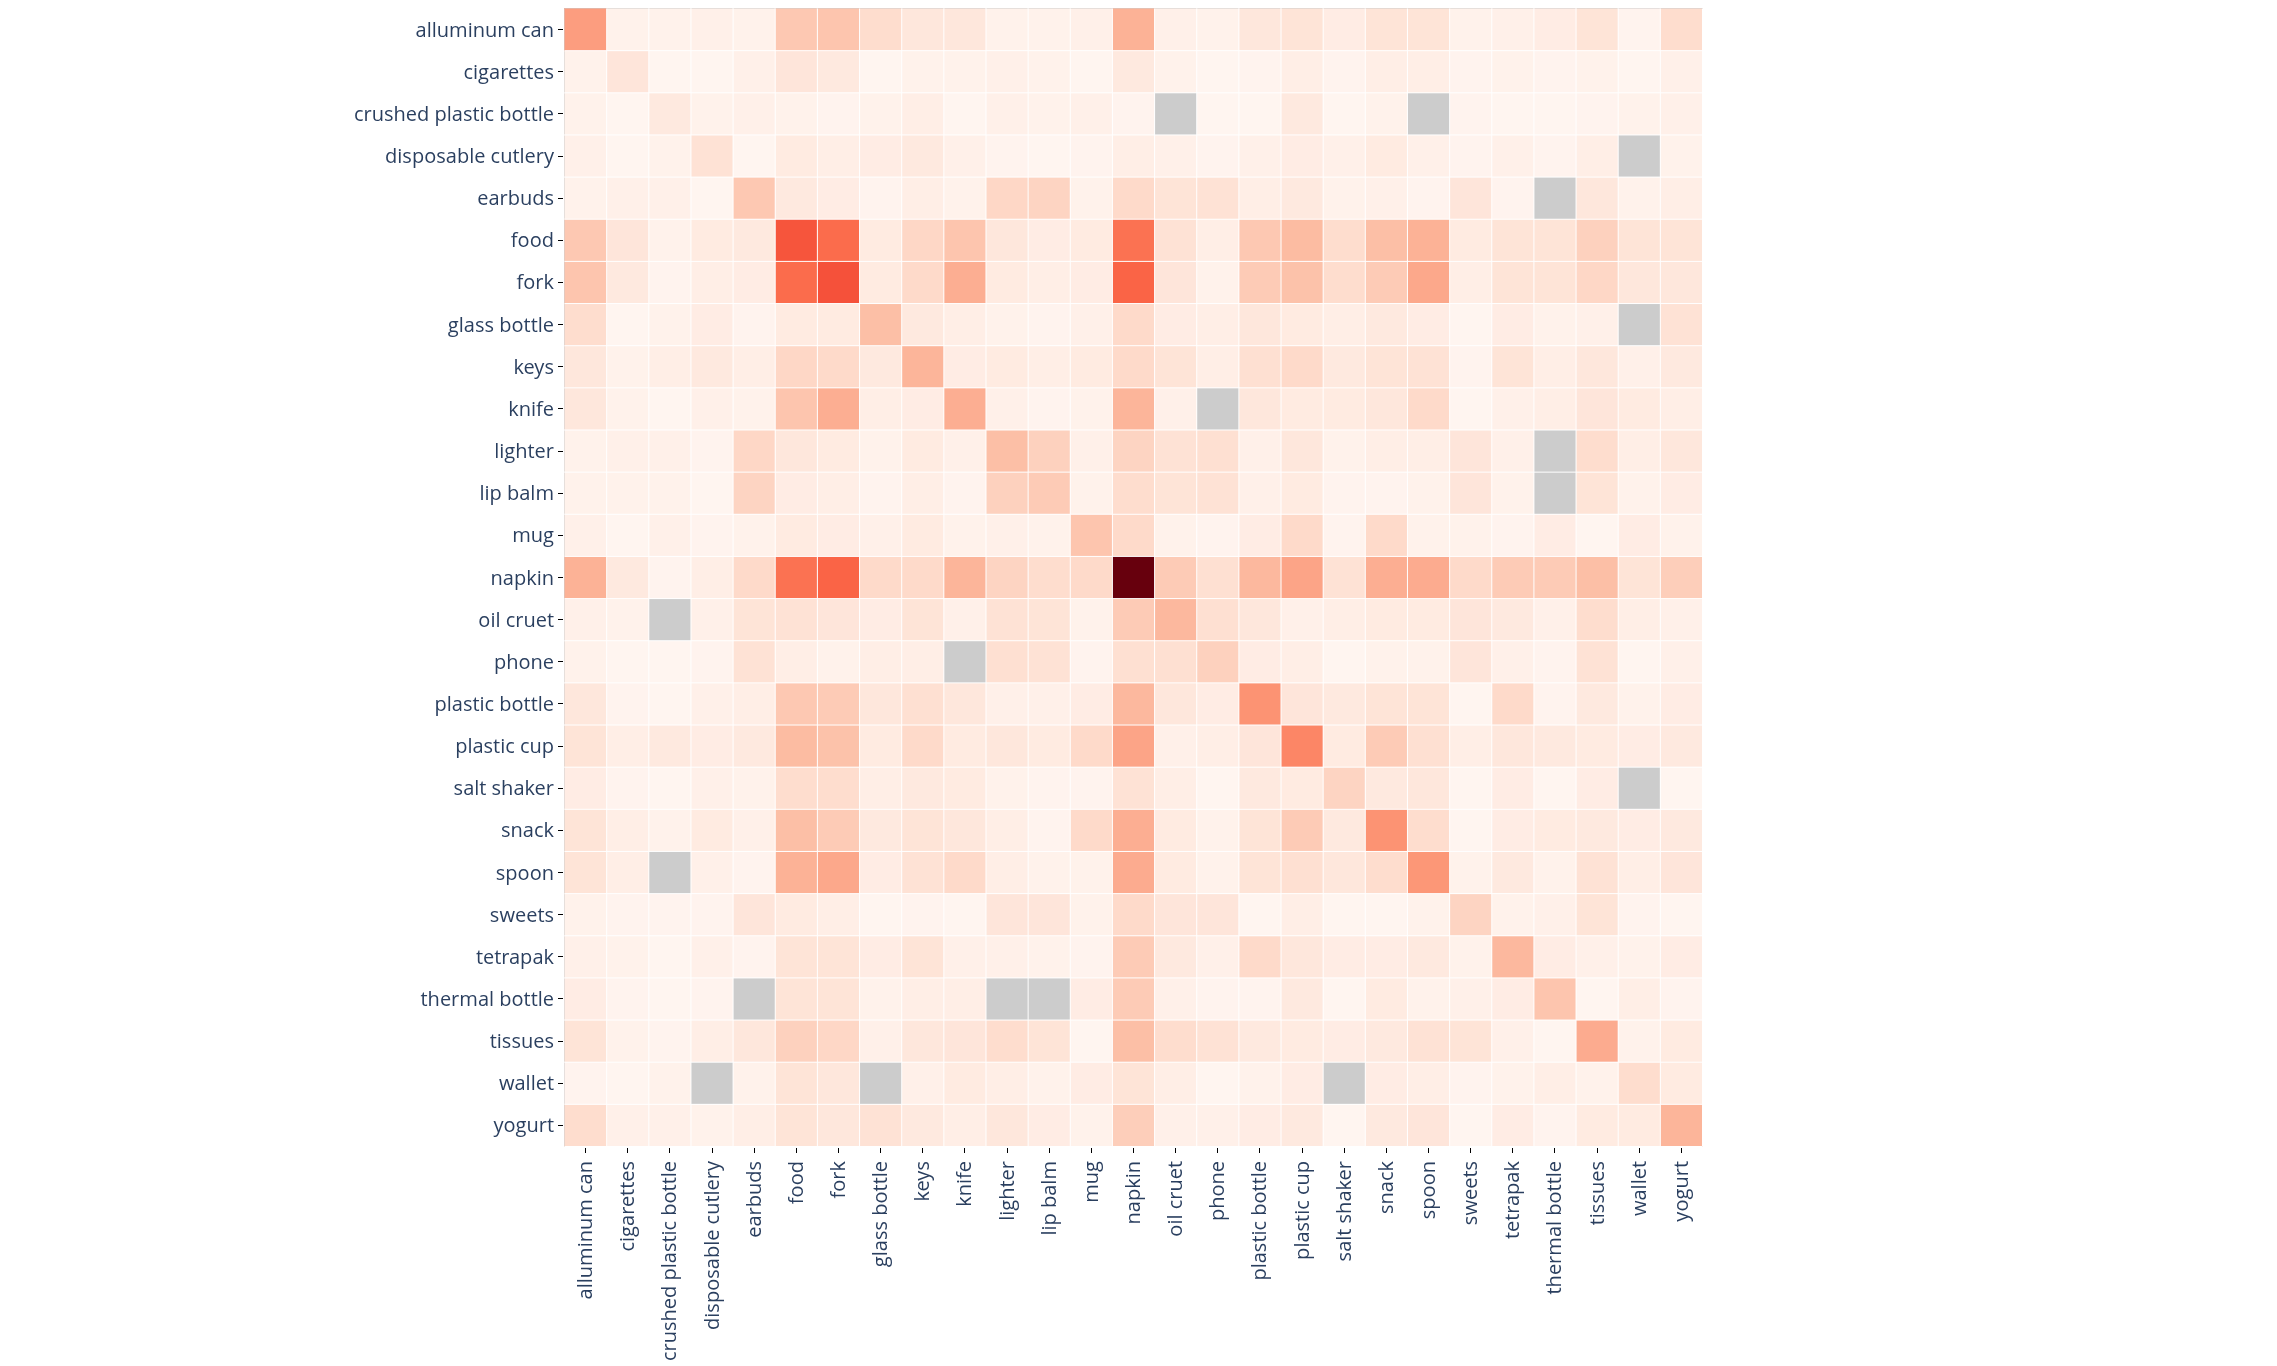
\includegraphics[width=\linewidth]{bin_full_ccm} 
\caption{La diagonale rappresenta il numero di foto in cui appare una classe; tutto il resto indica in quante foto distinte due classi siano apparse insieme. Il colore grigio indica che il valore è nullo.}
\label{fig:subim6}
\end{figure}

\begin{figure}[!ht]
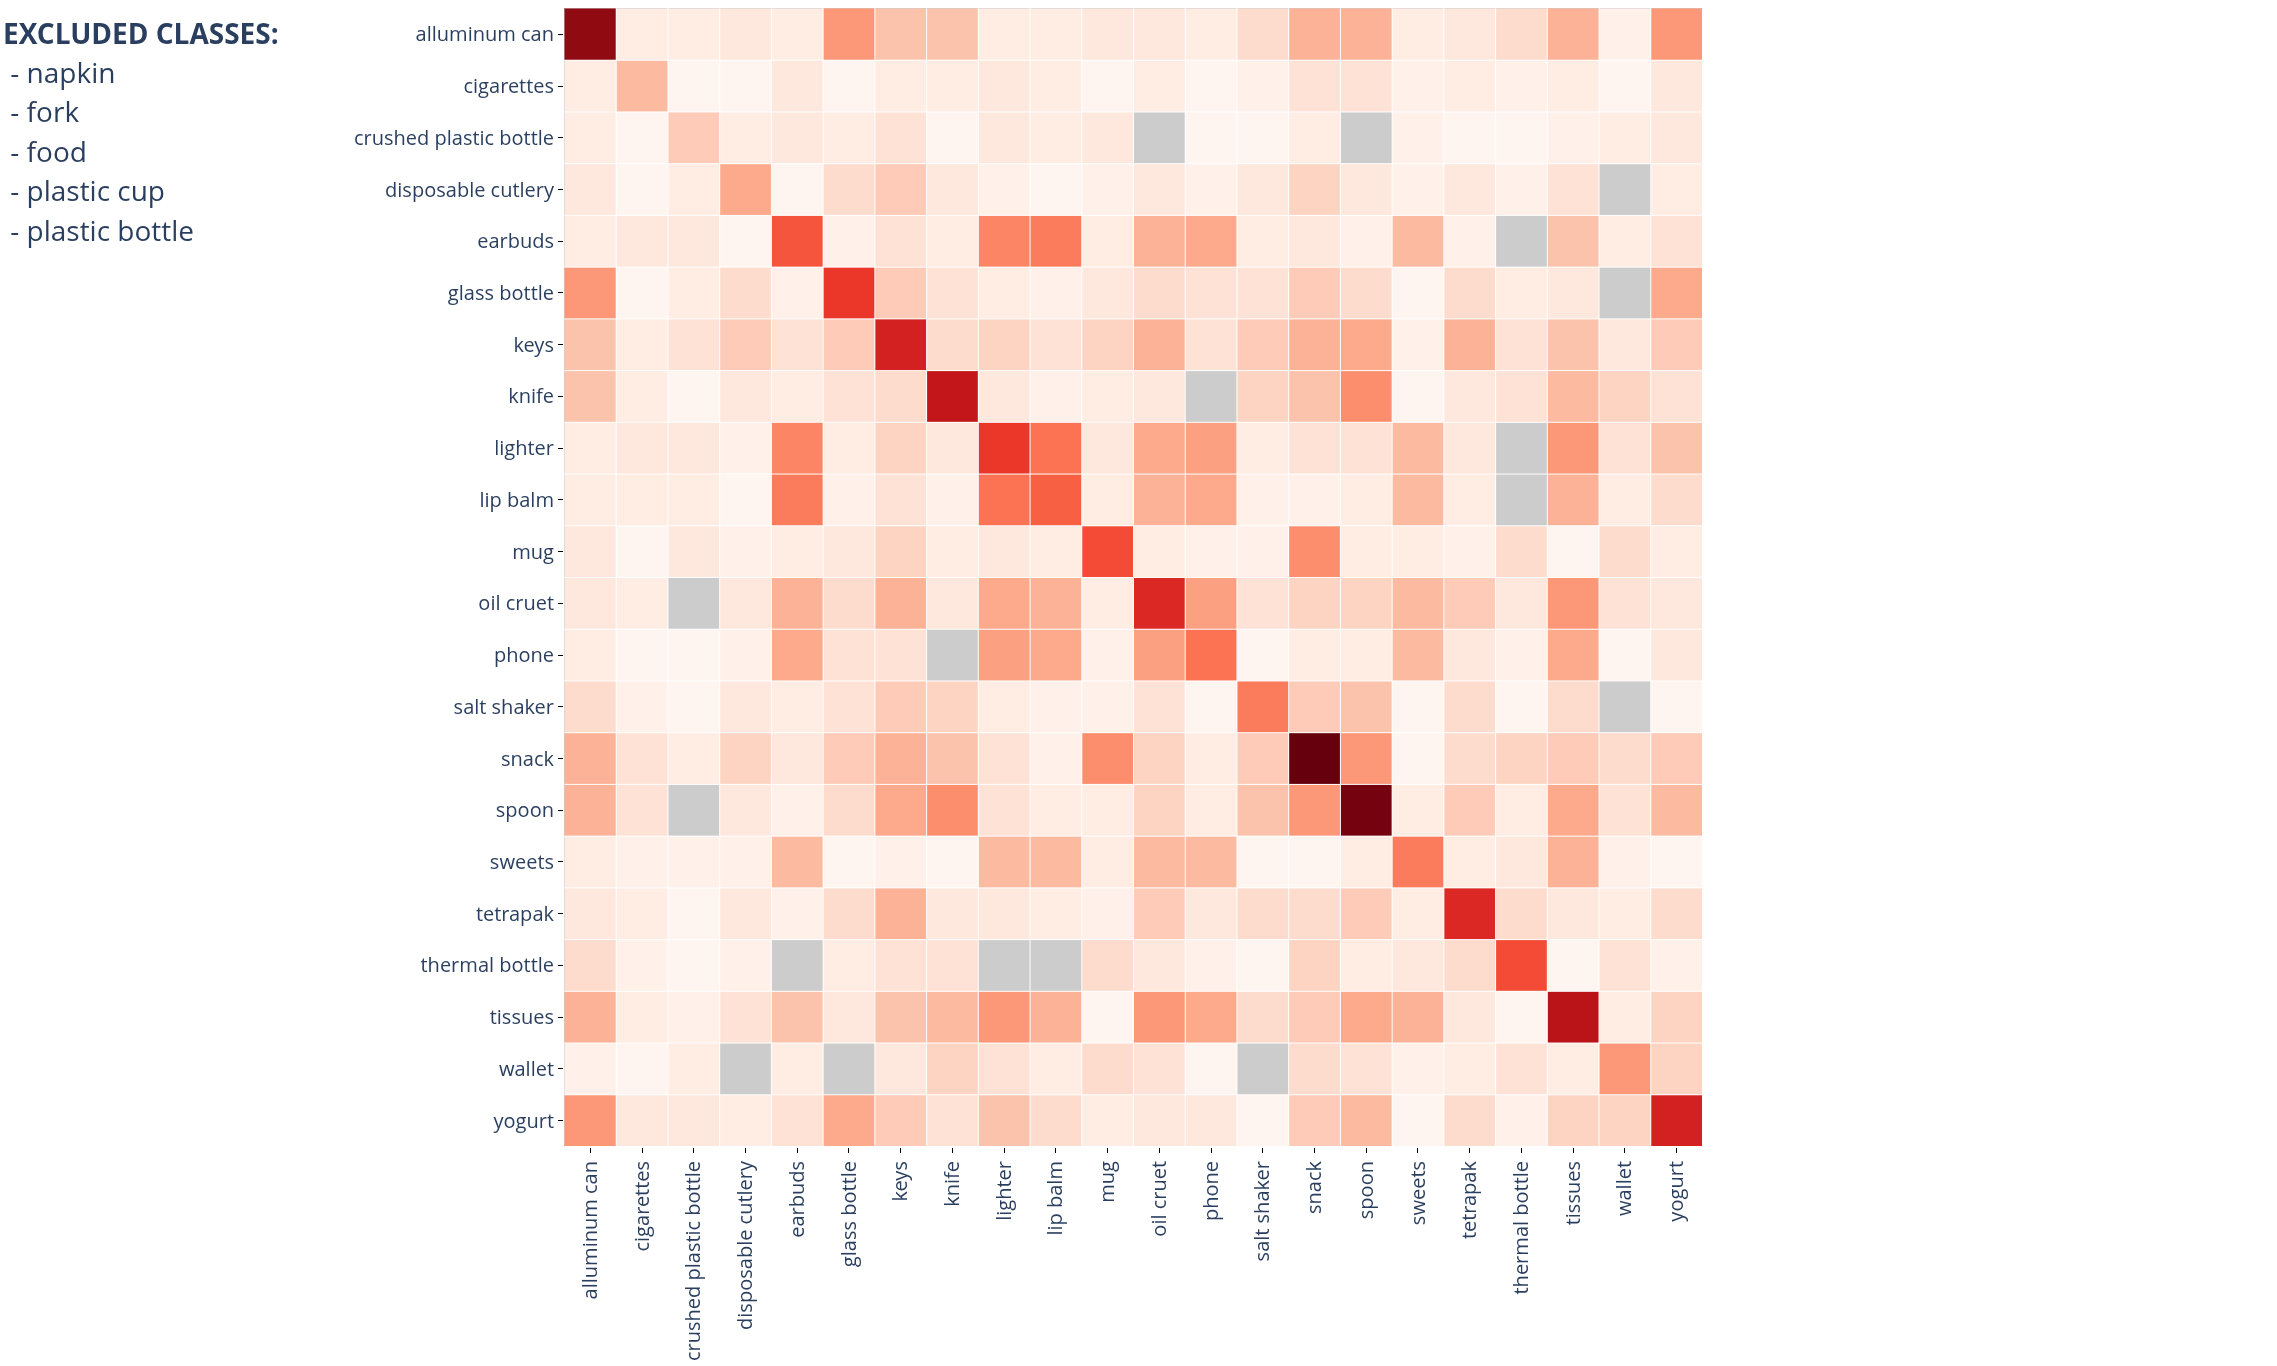
\includegraphics[width=\linewidth]{bin_partial_ccm} 
\label{fig:subim7}
\caption{Presenta la stessa informazione della figura \ref{fig:subim6}, rimuovendo le cinque classi che appaiano complessivamente in più foto (non che presentano il maggior numero di istanze).}
\end{figure}


\end{document}